\subsection{\RU{Инструкции}\EN{Instructions}}
\label{sec:x86_instructions}

\RU{Инструкции, отмеченные как (M) обычно не генерируются компилятором: если вы видите её, очень может быть
это вручную написанный фрагмент кода, либо это т.н. compiler intrinsic}
\EN{Instructions marked as (M) are not usually generated by the compiler: if you see one of them, it is probably
a hand-written piece of assembly code, or a compiler intrinsic} (\myref{sec:compiler_intrinsic}).

% TODO ? обратные инструкции

\RU{Только наиболее используемые инструкции перечислены здесь}
\EN{Only the most frequently used instructions are listed here}.
\EN{You can read \myref{x86_manuals} for a full documentation.}%
\RU{Обращайтесь к \myref{x86_manuals} для полной документации.}

\RU{Нужно ли заучивать опкоды инструкций на память?}\EN{Do you have to know all instruction's opcodes by heart?}
\RU{Нет, только те, которые часто используются для модификации кода}\EN{No, only those
which are used for code patching} (\myref{x86_patching}).
\RU{Остальные запоминать нет смысла.}\EN{All the rest of the opcodes don't need to be memorized.}

\subsubsection{\RU{Префиксы}\EN{Prefixes}}

\myindex{x86!\Prefixes!LOCK}
\myindex{x86!\Prefixes!REP}
\myindex{x86!\Prefixes!REPE/REPNE}
\begin{description}
\label{x86_lock}
\item[LOCK] \RU{используется чтобы предоставить эксклюзивный доступ к памяти в многопроцессорной среде}
\EN{forces CPU to make exclusive access to the RAM in multiprocessor environment}.
\RU{Для упрощения, можно сказать, что когда исполняется инструкция с этим префиксом, остальные процессоры
в системе останавливаются}\EN{For the sake of simplification, it can be said that when an instruction
with this prefix is executed, all other CPUs in a multiprocessor system are stopped}.
\RU{Чаще все это используется для критических секций, семафоров, мьютексов}\EN{Most often
it is used for critical sections, semaphores, mutexes}.
\RU{Обычно используется с}\EN{Commonly used with} ADD, AND, BTR, BTS, CMPXCHG, OR, XADD, XOR.
\RU{Читайте больше о критических секциях}\EN{You can read more about critical sections here} (\myref{critical_sections}).

\item[REP] \RU{используется с инструкциями}\EN{is used with the} MOVSx \AndENRU STOSx\EN{ instructions}:
\RU{инструкция будет исполняться в цикле, счетчик расположен в регистре CX/ECX/RCX}
\EN{execute the instruction in a loop, the counter is located in the CX/ECX/RCX register}.
\RU{Для более детального описания, читайте больше об инструкциях}
\EN{For a detailed description, read more about the} MOVSx (\myref{REP_MOVSx}) 
\AndENRU STOSx (\myref{REP_STOSx})\EN{ instructions}.

\RU{Работа инструкций с префиксом REP зависит от флага DF, он задает направление}
\EN{The instructions prefixed by REP are sensitive to the DF flag, which is used to set the direction}.

\item[REPE/REPNE] (\ac{AKA} REPZ/REPNZ) \RU{используется с инструкциями}\EN{used with} CMPSx \AndENRU
SCASx\EN{ instructions}:
\RU{инструкция будет исполняться в цикле, счетчик расположен в регистре \TT{CX}/\TT{ECX}/\TT{RCX}}
\EN{execute the last instruction in a loop, the count is set in the \TT{CX}/\TT{ECX}/\TT{RCX} register}. 
\RU{Выполнение будет прервано если ZF будет 0 (REPE) либо если ZF будет 1 (REPNE)}
\EN{It terminates prematurely if ZF is 0 (REPE) or if ZF is 1 (REPNE)}.

\RU{Для более детального описания, читайте больше об инструкциях}
\EN{For a detailed description, you can read more about the} CMPSx (\myref{REPE_CMPSx}) 
\AndENRU SCASx (\myref{REPNE_SCASx})\EN{ instructions}.

\RU{Работа инструкций с префиксами REPE/REPNE зависит от флага DF, он задает направление}
\EN{Instructions prefixed by REPE/REPNE are sensitive to the DF flag, which is used to set the direction}.

\end{description}

\subsubsection{\RU{Наиболее часто используемые инструкции}\EN{Most frequently used instructions}}

\RU{Их можно заучить в первую очередь}\EN{These can be memorized in the first place}.

\begin{description}
% in order to keep them easily sorted...
\input{appendix/x86/instructions/ADC}
\myindex{x86!\Instructions!ADD}
  \item[ADD] \RU{сложить два значения}\EN{add two values}\FR{ajoute deux valeurs}

\myindex{x86!\Instructions!AND}
  \item[AND] \RU{логическое \q{И}}\EN{logical \q{and}}\FR{\q{et} logique}

\myindex{x86!\Instructions!CALL}
  \item[CALL] \RU{вызвать другую функцию}\EN{call another function}\FR{appelle une autre fonction}:\\
  \TT{PUSH address\_after\_CALL\_instruction; JMP label}

\myindex{x86!\Instructions!CMP}
\myindex{x86!\Instructions!SUB}
  \item[CMP] \RU{сравнение значений и установка флагов, то же что и \TT{SUB}, но только без записи результата}
  \EN{compare values and set flags, the same as \TT{SUB} but without writing the result}
  \FR{compare les valeurs et met les flags, comme \TT{SUB} mais sans écrire le résultat}

\myindex{x86!\Instructions!DEC}
\myindex{x86!\Flags!CF}
  \item[DEC] \gls{decrement}.
\RU{В отличие от других арифметических инструкций, \TT{DEC} не модифицирует флаг CF.}%
\EN{Unlike other arithmetic instructions, \TT{DEC} doesn't modify CF flag.}%

\myindex{x86!\Instructions!IMUL}
  \item[IMUL] \RU{умножение с учетом знаковых значений}\EN{signed multiply}\FR{multiplication signée}
  \EN{\IMUL often used instead of \MUL, read more about it:}%
  \RU{\IMUL часто используется вместо \MUL, читайте об этом больше:}%
  \FR{\IMUL est souvent utilisé à la place de \MUL, voir ici:} \ref{IMUL_over_MUL}.


\myindex{x86!\Instructions!INC}
\myindex{x86!\Flags!CF}
  \item[INC] \gls{increment}.
\RU{В отличие от других арифметических инструкций, \TT{INC} не модифицирует флаг CF.}%
\EN{Unlike other arithmetic instructions, \TT{INC} doesn't modify CF flag.}

\myindex{x86!\Instructions!JCXZ}
\myindex{x86!\Instructions!JECXZ}
\myindex{x86!\Instructions!JRCXZ}
  \item[JCXZ, JECXZ, JRCXZ] (M) \RU{переход если CX/ECX/RCX=0}\EN{jump if CX/ECX/RCX=0}\FR{saute si CX/ECX/RCX=0}

\myindex{x86!\Instructions!JMP}
\item[JMP] \RU{перейти на другой адрес}\EN{jump to another address}\FR{saute à une
autre adresse}.
\RU{Опкод имеет т.н.}\EN{The opcode has a}\FR{L'opcode a un} \gls{jump offset}.

\item[Jcc] (\RU{где}\EN{where} cc\EMDASH{}condition code)

\myindex{x86!\Instructions!JAE}
\myindex{x86!\Instructions!JA}
\myindex{x86!\Instructions!JBE}
\myindex{x86!\Instructions!JB}
\myindex{x86!\Instructions!JC}
\myindex{x86!\Instructions!JE}
\myindex{x86!\Instructions!JGE}
\myindex{x86!\Instructions!JG}
\myindex{x86!\Instructions!JLE}
\myindex{x86!\Instructions!JL}
\myindex{x86!\Instructions!JNAE}
\myindex{x86!\Instructions!JNA}
\myindex{x86!\Instructions!JNBE}
\myindex{x86!\Instructions!JNB}
\myindex{x86!\Instructions!JNC}
\myindex{x86!\Instructions!JNE}
\myindex{x86!\Instructions!JNGE}
\myindex{x86!\Instructions!JNG}
\myindex{x86!\Instructions!JNLE}
\myindex{x86!\Instructions!JNL}
\myindex{x86!\Instructions!JNO}
\myindex{x86!\Instructions!JNS}
\myindex{x86!\Instructions!JNZ}
\myindex{x86!\Instructions!JO}
\myindex{x86!\Instructions!JPO}
\myindex{x86!\Instructions!JP}
\myindex{x86!\Instructions!JS}
\myindex{x86!\Instructions!JZ}

\RU{Немало этих инструкций имеют синонимы (отмечены с AKA), это сделано для удобства}
\EN{A lot of these instructions have synonyms (denoted with AKA), this was done for convenience}.
\RU{Синонимичные инструкции транслируются в один и тот же опкод}
\EN{Synonymous instructions are translated into the same opcode}.
\RU{Опкод имеет т.н.}\EN{The opcode has a} \gls{jump offset}.

\label{Jcc}
\begin{description}
\item[JAE] \ac{AKA} JNC: \RU{переход если больше или равно (беззнаковый)}\EN{jump if above or equal (unsigned)}: CF=0
\EN{\item[JA] \ac{AKA} JNBE: jump if greater (unsigned): CF=0 and ZF=0}
\RU{\item[JA] \ac{AKA} JNBE: переход если больше (беззнаковый): CF=0 и ZF=0}
\EN{\item[JBE] jump if lesser or equal (unsigned): CF=1 or ZF=1}
\RU{\item[JBE] переход если меньше или равно (беззнаковый): CF=1 или ZF=1}
\item[JB] \ac{AKA} JC: \RU{переход если меньше (беззнаковый)}\EN{jump if below (unsigned)}: CF=1
\item[JC] \ac{AKA} JB: \RU{переход если CF=1}\EN{jump if CF=1}
\item[JE] \ac{AKA} JZ: \RU{переход если равно или ноль}\EN{jump if equal or zero}: ZF=1
\item[JGE] \RU{переход если больше или равно (знаковый)}\EN{jump if greater or equal (signed)}: SF=OF
\EN{\item[JG] jump if greater (signed): ZF=0 and SF=OF}
\RU{\item[JG] переход если больше (знаковый): ZF=0 и SF=OF}
\EN{\item[JLE] jump if lesser or equal (signed): ZF=1 or SF$\neq$OF}
\RU{\item[JLE] переход если меньше или равно (знаковый): ZF=1 или SF$\neq$OF}
\item[JL] \RU{переход если меньше (знаковый)}\EN{jump if lesser (signed)}: SF$\neq$OF
\item[JNAE] \ac{AKA} JC: \RU{переход если не больше или равно (беззнаковый)}\EN{jump if not above or equal (unsigned)} CF=1
\item[JNA] \RU{переход если не больше (беззнаковый)}\EN{jump if not above (unsigned)} CF=1 \AndENRU ZF=1
\item[JNBE] \RU{переход если не меньше или равно (беззнаковый)}\EN{jump if not below or equal (unsigned)}: CF=0 \AndENRU ZF=0
\item[JNB] \ac{AKA} JNC: \RU{переход если не меньше (беззнаковый)}\EN{jump if not below (unsigned)}: CF=0
\item[JNC] \ac{AKA} JAE: \RU{переход если CF=0, синонимично}\EN{jump CF=0 synonymous to} JNB.
\item[JNE] \ac{AKA} JNZ: \RU{переход если не равно или не ноль}\EN{jump if not equal or not zero}: ZF=0
\item[JNGE] \RU{переход если не больше или равно (знаковый)}\EN{jump if not greater or equal (signed)}: SF$\neq$OF
\EN{\item[JNG] jump if not greater (signed): ZF=1 or SF$\neq$OF}
\RU{\item[JNG] переход если не больше (знаковый): ZF=1 или SF$\neq$OF}
\item[JNLE] \RU{переход если не меньше или равно (знаковый)}\EN{jump if not lesser or equal (signed)}: ZF=0 \AndENRU SF=OF
\item[JNL] \RU{переход если не меньше (знаковый)}\EN{jump if not lesser (signed)}: SF=OF
\item[JNO] \RU{переход если не переполнение}\EN{jump if not overflow}: OF=0
\item[JNS] \RU{переход если флаг SF сброшен}\EN{jump if SF flag is cleared}
\item[JNZ] \ac{AKA} JNE: \RU{переход если не равно или не ноль}\EN{jump if not equal or not zero}: ZF=0
\item[JO] \RU{переход если переполнение}\EN{jump if overflow}: OF=1
\item[JPO] \RU{переход если сброшен флаг PF}\EN{jump if PF flag is cleared} (Jump Parity Odd)
\item[JP] \ac{AKA} \ac{JPE}: \RU{переход если выставлен флаг PF}\EN{jump if PF flag is set}
\item[JS] \RU{переход если выставлен флаг SF}\EN{jump if SF flag is set}
\item[JZ] \ac{AKA} JE: \RU{переход если равно или ноль}\EN{jump if equal or zero}: ZF=1
\end{description}


\myindex{x86!\Instructions!LAHF}
\myindex{x86!\Registers!AH}
  \item[LAHF] \RU{скопировать биты флагов статуса в AH}\EN{copy status flag bits to AH}:

\input{SAHF_LAHF}

\RU{Эта инструкция часто используется в коде работающем с \ac{FPU}.}
\EN{This instruction is often used in \ac{FPU}-related code.}


\myindex{x86!\Instructions!LEAVE}
\label{x86_ins:LEAVE}
\item[LEAVE] \RU{аналог команд \TT{MOV ESP, EBP} и \TT{POP EBP}\EMDASH{}
то есть возврат \glslink{stack pointer}{указателя стека} и регистра \EBP в первоначальное состояние.}%
\EN{equivalent of the \TT{MOV ESP, EBP} and \TT{POP EBP} instruction
pair\EMDASH{}in other words, this instruction sets the \gls{stack pointer} (\ESP) back and restores
the \EBP register to its initial state.}%
\FR{équivalente à la paire d'instructions  \TT{MOV ESP, EBP} et \TT{POP EBP} \EMDASH{}autrement dit,
cette instruction remet le \glslink{stack pointer}{pointeur de pile} et restaure le registre
\EBP à l'état initial.}


\input{appendix/x86/instructions/LEA}
\input{appendix/x86/instructions/MOVSB_W_D_Q}
\myindex{x86!\Instructions!MOVSX}
  \item[MOVSX] \RU{загрузить с расширением знака}\EN{load with sign extension}\FR{charger avec extension du signe}%
  \RU{см. также}\EN{see also}\FR{voir aussi}: (\myref{MOVSX})

\myindex{x86!\Instructions!MOVZX}
  \item[MOVZX] \RU{загрузить и очистить все остальные биты}\EN{load and clear all other bits}i%
  \FR{charger et effacer tous les autres bits} \RU{см. также}\EN{see also}\FR{voir aussi}: (\myref{movzx})

\input{appendix/x86/instructions/MOV}
\myindex{x86!\Instructions!MUL}
  \item[MUL] \RU{умножение с учетом беззнаковых значений}\EN{unsigned multiply}\FR{multiplier sans signe}.
  \EN{\IMUL often used instead of \MUL, read more about it:}%
  \RU{\IMUL часто используется вместо \MUL, читайте об этом больше:}%
  \FR{\IMUL est souvent utilisée au lieu de \MUL, en lire plus ici:} \ref{IMUL_over_MUL}.


\myindex{x86!\Instructions!NEG}
  \item[NEG] \RU{смена знака}\EN{negation}\FR{négation}: $op=-op$
\EN{Same as \TT{NOT op / ADD op, 1}.}%
\RU{То же что и \TT{NOT op / ADD op, 1}.}%
\FR{La même chose que \TT{NOT op / ADD op, 1}.}


\input{appendix/x86/instructions/NOP}
\myindex{x86!\Instructions!NOT}
  \item[NOT] op1: $op1=\neg{}op1$. \FR{inversion logique}\RU{логическое \q{НЕ}}\EN{logical inversion}
  \RU{Важная особенность --- инструкция не меняет флаги.}%
  \EN{Important feature---the instruction doesn't change flags.}%
  \FR{Caractéristique importante---l'instruction ne change pas les flags.}

\myindex{x86!\Instructions!OR}
  \item[OR] \RU{логическое \q{ИЛИ}}\EN{logical \q{or}}\FR{\q{ou} logique}

\myindex{x86!\Instructions!POP}
\EN{\item[POP] get a value from the stack: \TT{value=SS:[ESP]; ESP=ESP+4 (or 8)}}%
\RU{\item[POP] взять значение из стека: \TT{value=SS:[ESP]; ESP=ESP+4 (или 8)}}%
\FR{\item[POP] prend une valeur depuis la pile: \TT{value=SS:[ESP]; ESP=ESP+4 (ou 8)}}


\myindex{x86!\Instructions!PUSH}
\EN{\item[PUSH] push a value into the stack: \TT{ESP=ESP-4 (or 8); SS:[ESP]=value}}%
\RU{\item[PUSH] записать значение в стек: \TT{ESP=ESP-4 (или 8); SS:[ESP]=value}}%
\FR{\item[PUSH] pousse une valeur sur la pile: \TT{ESP=ESP-4 (ou 8); SS:[ESP]=value}}


\input{appendix/x86/instructions/RET}
\myindex{x86!\Instructions!SAHF}
\myindex{x86!\Registers!AH}

  \item[SAHF] \RU{скопировать биты из AH в флаги CPU}\EN{copy bits from AH to CPU flags}%
  \FR{copier des bits de AH vers les flags CPU}:

\input{SAHF_LAHF}

\RU{Эта инструкция часто используется в коде работающем с \ac{FPU}.}%
\EN{This instruction is often used in \ac{FPU}-related code.}%
\FR{Cette instruction est souvent utilisée dans du code relatif au \ac{FPU}.}


\myindex{x86!\Instructions!SBB}
\myindex{x86!\Flags!CF}
  \item[SBB] (\IT{subtraction with borrow}) 
  \RU{вычесть одно значение из другого, \glslink{decrement}{декремент} результата если флаг CF выставлен.
  SBB часто используется для вычитания больших значений, например, для вычитания двух 64-битных
  значений в 32-битной среде используя инструкции SUB и SBB, например:}
  \EN{subtract values, \gls{decrement} the result if the CF flag is set.
  SBB is often used for subtraction of large values, for example,
  to subtract two 64-bit values in 32-bit environment using two SUB and SBB instructions. For example:}
  \FR{soustrait les valeurs, \glslink{decrement}{décrémente} le résultat si le flag
  CF est mis. SBB est souvent utilisé pour la soustraction de grandes valeurs, par
  exemple:}

\EN{\lstinputlisting[style=customasmx86]{appendix/x86/instructions/SBB_example_EN.lst}}
\RU{\lstinputlisting[style=customasmx86]{appendix/x86/instructions/SBB_example_RU.lst}}
\FR{\lstinputlisting[style=customasmx86]{appendix/x86/instructions/SBB_example_FR.lst}}

\RU{Еще один пример}\EN{One more example}\FR{Un autre exemple}: \myref{sec:64bit_in_32_env}.

\input{appendix/x86/instructions/SCASB_W_D_Q}
\myindex{x86!\Instructions!SHL}
\myindex{x86!\Instructions!SHR}
  \item[SHL] \RU{сдвинуть значение влево}\EN{shift value left}\FR{décale une valeur à gauche}
  \item[SHR] \RU{сдвинуть значение вправо}\EN{shift value right}\FR{décale une valeur à droite}:

\input{shift_left}
\input{shift_right}

  \RU{Эти инструкции очень часто применяются для умножения и деления на}\EN{These instructions are frequently
  used for multiplication and division by}\FR{Ces instructions sont utilisées fréquemment
  pour la multiplication et la division par} $2^n$.
  \RU{Еще одно очень частое применение это работа с битовыми полями}%
  \EN{Another very frequent application is processing bit fields}%
  \FR{Une autre utilisation très fréquente est le traitement des champs de bits}: \myref{sec:bitfields}.

\myindex{x86!\Instructions!SHRD}
\item[SHRD] op1, op2, op3: \RU{сдвинуть значение в op2 вправо на op3 бит, подтягивая
биты из op1}%
\EN{shift value in op2 right by op3 bits, taking bits from op1}%
\FR{décale la valeur dans op2 de op3 bits vers la droite, en prenant les bits depuis op1}.

% TODO: picture

\Example: \myref{sec:64bit_in_32_env}.

\input{appendix/x86/instructions/STOSB_W_D_Q}
\myindex{x86!\Instructions!SUB}
  \item[SUB] \RU{вычесть одно значение из другого. 
  часто встречающийся вариант \TT{SUB reg,reg} означает обнуление \IT{reg}.}
  \EN{subtract values. 
  A frequently occurring pattern is \TT{SUB reg,reg}, which implies zeroing of \IT{reg}.}
  \FR{soustrait des valeurs.
  Une utilisation fréquente est \TT{SUB reg,reg}, qui met \IT{reg} à zéro.}

\myindex{x86!\Instructions!TEST}
\myindex{x86!\Instructions!AND}
  \item[TEST] \RU{то же что и AND, но без записи результатов, см. также}%
\EN{same as AND but without saving the result, see also}%
\FR{comme AND mais sans sauvegarder le résultat, voir aussi}: \myref{sec:bitfields}

\myindex{x86!\Instructions!XOR}
  \item[XOR] op1, op2: \ac{XOR} \RU{значений}\EN{values}\FR{valeurs}. $op1=op1\oplus{}op2$.
  \RU{Часто встречающийся вариант \TT{XOR reg,reg} означает обнуление регистра \IT{reg}.}
  \EN{A frequently occurring pattern is \TT{XOR reg,reg}, which implies zeroing of \IT{reg}.}
  \FR{Un schéma récurrent est \TT{XOR reg,reg}, qui met \IT{reg} à zéro.}
  \EN{See also}\RU{См.также}\FR{Voir aussi}: \myref{XOR_property}.


\end{description}

\subsubsection{\RU{Реже используемые инструкции}\EN{Less frequently used instructions}}

\begin{description}
\myindex{x86!\Instructions!BSF}
  \item[BSF] \IT{bit scan forward}, \RU{см. также}\EN{see also}\FR{voir aussi}: \myref{instruction_BSF}

\input{appendix/x86/instructions/BSR}
\myindex{x86!\Instructions!BSWAP}
  \item[BSWAP] \IT{(byte swap)}, \RU{смена \glslink{endianness}{порядка байт} в значении}\EN{change value \gls{endianness}}%
  \FR{change le \glslink{endianness}{boutisme} de la valeur}.

\input{appendix/x86/instructions/BTC}
\input{appendix/x86/instructions/BTR}
\input{appendix/x86/instructions/BTS}
\input{appendix/x86/instructions/BT}
\input{appendix/x86/instructions/CBW_CWDE_CDQ}
\myindex{x86!\Instructions!CLD}
\myindex{x86!\Flags!DF}
  \item[CLD] \RU{сбросить флаг DF}\EN{clear DF flag}\FR{éfface le flag DF}.

\myindex{x86!\Instructions!CLI}
\myindex{x86!\Flags!IF}
  \item[CLI] (M) \RU{сбросить флаг IF}\EN{clear IF flag}\FR{éfface le flag IF}.

\myindex{x86!\Instructions!CMC}
\myindex{x86!\Flags!CF}
  \item[CMC] (M) \RU{инвертировать флаг CF}\EN{toggle CF flag}\FR{bascule le flag CF}

\input{appendix/x86/instructions/CMOVcc}
\input{appendix/x86/instructions/CMPSB_W_D_Q}
\myindex{x86!\Instructions!CPUID}
  \item[CPUID] \RU{получить информацию о доступных возможностях \ac{CPU}}
  \EN{get information about the \ac{CPU}'s features}\FR{renvoie des informations
sur les fonctionnalités du \ac{CPU}}.
\RU{см. также}\EN{see also}\FR{Voir aussi}: (\myref{cpuid}).


\myindex{x86!\Instructions!DIV}
  \item[DIV] \RU{деление с учетом беззнаковых значений}\EN{unsigned division}\FR{division non signée}

\myindex{x86!\Instructions!IDIV}
  \item[IDIV] \RU{деление с учетом знаковых значений}\EN{signed division}\FR{division signée}

\input{appendix/x86/instructions/INT}
\myindex{x86!\Instructions!IN}
\myindex{MS-DOS}
  \item[IN] (M) \RU{получить данные из порта}\EN{input data from port}\FR{lire des données depuis le port}.
	  \RU{Эту инструкцию обычно можно найти в драйверах OS либо в старом коде для MS-DOS,
	  например}%
	  \EN{The instruction usually can be seen in OS drivers or in old MS-DOS code,
	  for example}%
      \FR{On trouve cettte instruction dans les drivers de l'OS ou dans de l'ancien
      code MS-DOS, par exemple} (\myref{IN_example}).

\myindex{x86!\Instructions!IRET}
\myindex{MS-DOS}

\item[IRET]: \RU{использовалась в среде MS-DOS для возврата из обработчика прерываний,
после того как он был вызван при помощи инструкции INT}
\EN{was used in the MS-DOS environment for returning from an interrupt handler after it was
called by the INT instruction}\FR{était utilisée dans l'environnement MS-DOS pour
retourner d'un gestionnaire d'interruption appelé par l'instruction INT}.
\RU{Эквивалентна}\EN{Equivalent to}\FR{Équivalent à} \TT{POP tmp; POPF; JMP tmp}.


\input{appendix/x86/instructions/LOOP}
\myindex{x86!\Instructions!OUT}
\myindex{MS-DOS}
  \item[OUT] (M) \RU{послать данные в порт}\EN{output data to port}\FR{encoie des données sur le port}.
	  \RU{Эту инструкцию обычно можно найти в драйверах OS либо в старом коде для MS-DOS,
	  например}%
	  \EN{The instruction usually can be seen in OS drivers or in old MS-DOS code,
	  for example}%
      \FR{L'instruction peut être vue, en général, dans les drivers d'OS ou dans
      du vieux code MS-DOS, par exemple} (\myref{OUT_example}).

\myindex{x86!\Instructions!POPA}
  \item[POPA] (M) \RU{восстанавливает значения регистров}\EN{restores values of}\FR{restaure les valeurs des registres}
  (R|E)DI, (R|E)SI, (R|E)BP, (R|E)BX, (R|E)DX, (R|E)CX, (R|E)AX \RU{из стека}\EN{registers from the stack}\FR{depuis la pile}.


\myindex{x86!\Instructions!POPCNT}
  \item[POPCNT] population count. \RU{Считает количество бит выставленных в 1 в значении}
  \EN{Counts the number of 1 bits in the value}\FR{Compte le nombre de bits à 1 dans la valeur}.

  \EN{See: \myref{POPCNT}.}
  % TODO russian translation
  \FR{Voir: \myref{POPCNT}.}



\myindex{x86!\Instructions!POPF}
  \item[POPF] \RU{восстановить флаги из стека}\EN{restore flags from the stack}\FR{restaure
  les flags depuis la pile} (\ac{AKA} \RU{регистр EFLAGS}\EN{EFLAGS register}\FR{registre EFLAGS})

\myindex{x86!\Instructions!PUSHA}
  \item[PUSHA] (M) \RU{сохраняет значения регистров}\EN{pushes the values of the}\FR{pousse
  les valeurs des registres}
  (R|E)AX, (R|E)CX, (R|E)DX, (R|E)BX, (R|E)BP, (R|E)SI, (R|E)DI \RU{в стеке}\EN{registers
  to the stack}\FR{sur la pile}.

\myindex{x86!\Instructions!PUSHF}
  \item[PUSHF] \RU{сохранить в стеке флаги}\EN{push flags}\FR{pousse les flags} (\ac{AKA}
  \RU{регистр EFLAGS}\EN{EFLAGS register}\FR{registre EFLAGS})


\myindex{x86!\Instructions!RCL}
\myindex{x86!\Instructions!RCR}
\myindex{x86!\Flags!CF}

  \item[RCL] (M) \RU{вращать биты налево через флаг CF}\EN{rotate left via CF flag}\FR{pivote vers la gauche via le flag CF}:

\begin{center}
	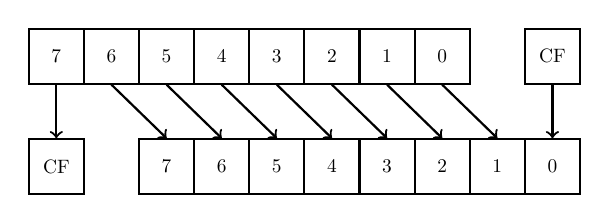
\begin{tikzpicture}[scale=0.7, every node/.style={scale=0.7}]
	\edef\bitsize{1cm}
	\tikzstyle{byte}=[draw,minimum size=\bitsize]
	\tikzstyle{every path}=[thick]

	\node [draw,rectangle,minimum size=\bitsize] (a1) {7};
	\node [draw,rectangle,minimum size=\bitsize] (a2) [right of=a1] {6};
	\node [draw,rectangle,minimum size=\bitsize] (a3) [right of=a2] {5};
	\node [draw,rectangle,minimum size=\bitsize] (a4) [right of=a3] {4};
	\node [draw,rectangle,minimum size=\bitsize] (a5) [right of=a4] {3};
	\node [draw,rectangle,minimum size=\bitsize] (a6) [right of=a5] {2};
	\node [draw,rectangle,minimum size=\bitsize] (a7) [right of=a6] {1};
	\node [draw,rectangle,minimum size=\bitsize] (a8) [right of=a7] {0};
	\node (empty1) [right of=a8] {};
	\node [rectangle,draw,minimum size=\bitsize] (acf) [right of=empty1] {CF};

	\node (empty) [below of=a1] {};

	\node [rectangle,draw,minimum size=\bitsize] (bcf) [below of=empty] {CF};
	\node (empty2) [right of=bcf] {};
	\node [draw,rectangle,minimum size=\bitsize] (b1) [right of=empty2] {7};
	\node [draw,rectangle,minimum size=\bitsize] (b2) [right of=b1] {6};
	\node [draw,rectangle,minimum size=\bitsize] (b3) [right of=b2] {5};
	\node [draw,rectangle,minimum size=\bitsize] (b4) [right of=b3] {4};
	\node [draw,rectangle,minimum size=\bitsize] (b5) [right of=b4] {3};
	\node [draw,rectangle,minimum size=\bitsize] (b6) [right of=b5] {2};
	\node [draw,rectangle,minimum size=\bitsize] (b7) [right of=b6] {1};
	\node [draw,rectangle,minimum size=\bitsize] (b8) [right of=b7] {0};

	\draw [->] (a1.south) -- (bcf.north); % 7
	\draw [->] (a2.south) -- (b1.north); % 6
	\draw [->] (a3.south) -- (b2.north);
	\draw [->] (a4.south) -- (b3.north);
	\draw [->] (a5.south) -- (b4.north);
	\draw [->] (a6.south) -- (b5.north);
	\draw [->] (a7.south) -- (b6.north);
	\draw [->] (a8.south) -- (b7.north);
	\draw [->] (acf.south) -- (b8.north);

	\end{tikzpicture}
\end{center}

  \item[RCR] (M) \RU{вращать биты направо через флаг CF}\EN{rotate right via CF flag}\FR{pivote vers la droite via le flag CF}:

\begin{center}
	\begin{tikzpicture}[scale=0.7, every node/.style={scale=0.7}]
	\edef\bitsize{1cm}
	\tikzstyle{byte}=[draw,minimum size=\bitsize]
	\tikzstyle{every path}=[thick]

	\node [rectangle,draw,minimum size=\bitsize] (acf) {CF};
	\node (empty1) [right of=acf] {};

	\node [draw,rectangle,minimum size=\bitsize] (a1) [right of=empty1] {7};
	\node [draw,rectangle,minimum size=\bitsize] (a2) [right of=a1] {6};
	\node [draw,rectangle,minimum size=\bitsize] (a3) [right of=a2] {5};
	\node [draw,rectangle,minimum size=\bitsize] (a4) [right of=a3] {4};
	\node [draw,rectangle,minimum size=\bitsize] (a5) [right of=a4] {3};
	\node [draw,rectangle,minimum size=\bitsize] (a6) [right of=a5] {2};
	\node [draw,rectangle,minimum size=\bitsize] (a7) [right of=a6] {1};
	\node [draw,rectangle,minimum size=\bitsize] (a8) [right of=a7] {0};

	\node (empty) [below of=a1] {};

	\node [draw,rectangle,minimum size=\bitsize] (b1) [below of=empty] {7};
	\node [draw,rectangle,minimum size=\bitsize] (b2) [right of=b1] {6};
	\node [draw,rectangle,minimum size=\bitsize] (b3) [right of=b2] {5};
	\node [draw,rectangle,minimum size=\bitsize] (b4) [right of=b3] {4};
	\node [draw,rectangle,minimum size=\bitsize] (b5) [right of=b4] {3};
	\node [draw,rectangle,minimum size=\bitsize] (b6) [right of=b5] {2};
	\node [draw,rectangle,minimum size=\bitsize] (b7) [right of=b6] {1};
	\node [draw,rectangle,minimum size=\bitsize] (b8) [right of=b7] {0};

	\node (empty2) [right of=b7] {};

	\node [rectangle,draw,minimum size=\bitsize] (bcf) [right=of empty2] {CF};

	\draw [->] (acf.south) -- (b1.north);
	\draw [->] (a1.south) -- (b2.north);
	\draw [->] (a2.south) -- (b3.north);
	\draw [->] (a3.south) -- (b4.north);
	\draw [->] (a4.south) -- (b5.north);
	\draw [->] (a5.south) -- (b6.north);
	\draw [->] (a6.south) -- (b7.north);
	\draw [->] (a7.south) -- (b8.north);
	\draw [->] (a8.south) -- (bcf.north);

	\end{tikzpicture}
\end{center}


\input{appendix/x86/instructions/ROx}
\myindex{x86!\Instructions!SAL}
  \item[SAL] \RU{Арифметический сдвиг влево}\EN{Arithmetic shift left}\FR{Décalager
  arithmétique à gauche}, \RU{синонимично}\EN{synonymous to}\FR{synonyme de} \TT{SHL}

\myindex{x86!\Instructions!SAR}
  \label{ins:SAR}
  \item[SAR] \RU{Арифметический сдвиг вправо}\EN{Arithmetic shift right}\FR{Décalage arithmétique à droite}

\begin{center}
	\begin{tikzpicture}[scale=0.7, every node/.style={scale=0.7}]
	\edef\bitsize{1cm}
	\tikzstyle{byte}=[draw,minimum size=\bitsize]
	\tikzstyle{every path}=[thick]

	\node [draw,rectangle,minimum size=\bitsize] (a1) {7};
	\node [draw,rectangle,minimum size=\bitsize] (a2) [right of=a1] {6};
	\node [draw,rectangle,minimum size=\bitsize] (a3) [right of=a2] {5};
	\node [draw,rectangle,minimum size=\bitsize] (a4) [right of=a3] {4};
	\node [draw,rectangle,minimum size=\bitsize] (a5) [right of=a4] {3};
	\node [draw,rectangle,minimum size=\bitsize] (a6) [right of=a5] {2};
	\node [draw,rectangle,minimum size=\bitsize] (a7) [right of=a6] {1};
	\node [draw,rectangle,minimum size=\bitsize] (a8) [right of=a7] {0};

	\node (empty) [below of=a1] {};

	\node [draw,rectangle,minimum size=\bitsize] (b1) [below of=empty] {7};
	\node [draw,rectangle,minimum size=\bitsize] (b2) [right of=b1] {6};
	\node [draw,rectangle,minimum size=\bitsize] (b3) [right of=b2] {5};
	\node [draw,rectangle,minimum size=\bitsize] (b4) [right of=b3] {4};
	\node [draw,rectangle,minimum size=\bitsize] (b5) [right of=b4] {3};
	\node [draw,rectangle,minimum size=\bitsize] (b6) [right of=b5] {2};
	\node [draw,rectangle,minimum size=\bitsize] (b7) [right of=b6] {1};
	\node [draw,rectangle,minimum size=\bitsize] (b8) [right of=b7] {0};

	\node [shape=rectangle,draw,minimum size=\bitsize] (cf) [right=of b7] {CF};

	\draw [->] (a1.south) -- (b1.north); %7
	\draw [->] (a1.south) -- (b2.north); %6

	\draw [->] (a2.south) -- (b3.north); %6
	\draw [->] (a3.south) -- (b4.north); %5
	\draw [->] (a4.south) -- (b5.north); %4
	\draw [->] (a5.south) -- (b6.north); %3
	\draw [->] (a6.south) -- (b7.north); %2
	\draw [->] (a7.south) -- (b8.north); %1

	\draw [->] (a8.south) -- (cf.north);

	\end{tikzpicture}
\end{center}

\RU{Таким образом, бит знака всегда остается на месте}%
\EN{Hence, the sign bit always stays at the place of the}%
\FR{De ce fait, le bit de signe reste toujours à la place du} \ac{MSB}.


\myindex{x86!\Instructions!SETcc}
  \item[SETcc] op: \RU{загрузить 1 в op (только байт) если условие верно или 0 если наоборот}%
  \EN{load 1 to operand (byte only) if the condition is true or zero otherwise}%
  \FR{charge 1 dans l'opérande (octet seulement) si la condition est vraie et zéro sinon}.
  \RU{Коды точно такие же, как и в инструкциях Jcc}\EN{The condition codes are the same as in the Jcc instructions}%
  \FR{Les codes conditions sont les même que les instructions Jcc}
  (\myref{Jcc}).


\myindex{x86!\Instructions!STC}
\myindex{x86!\Flags!CF}
  \item[STC] (M) \RU{установить флаг CF}\EN{set CF flag}\FR{met le flag CF}

\input{appendix/x86/instructions/STD}
\myindex{x86!\Instructions!STI}
\myindex{x86!\Flags!IF}
  \item[STI] (M) \RU{установить флаг IF}\EN{set IF flag}\FR{met le flag IF}

\myindex{x86!\Instructions!SYSCALL}
  \item[SYSCALL] (AMD) \RU{вызов сисколла}\EN{call syscall}\FR{appelle un appel système} (\myref{syscalls})

\myindex{x86!\Instructions!SYSENTER}
  \item[SYSENTER] (Intel) \RU{вызов сисколла}\EN{call syscall}\FR{appel un appel système} (\myref{syscalls})

\myindex{x86!\Instructions!UD2}
  \item[UD2] (M) \RU{неопределенная инструкция, вызывает исключение. Применяется для тестирования.}
  \EN{undefined instruction, raises exception. Used for testing.}\FR{instruction
  indéfinie, lève une exception. Utilisée pour tester.}

\myindex{x86!\Instructions!XCHG}
  \item[XCHG] (M) \RU{обменять местами значения в операндах}\EN{exchange the values in the operands}%
\FR{échange les valeurs dans les opérandes}

\myindex{Borland Delphi}
\RU{Это редкая инструкция: компиляторы её не генерируют, потому что начиная с Pentium, XCHG с адресом в памяти в операнде
исполняется так, как если имеет префикс LOCK (см.\InSqBrackets{\MAbrash глава 19}).
Вероятно, в Intel так сделали для совместимости с синхронизирующими примитивами.
Таким образом, XCHG начиная с Pentium может быть медленной.
С другой стороны, XCHG была очень популярна у программистов на ассемблере.
Так что, если вы видите XCHG в коде, это может быть знаком, что код написан вручную.
Впрочем, по крайней мере компилятор Borland Delphi генерирует эту инструкцию.}
\EN{This instruction is rare: compilers don't generate it, because starting at Pentium, XCHG with address in memory in operand executes as if it has LOCK prefix (\InSqBrackets{\MAbrash chapter 19}).
Perhaps, Intel engineers did so for compatibility with synchronizing primitives.
Hence, XCHG starting at Pentium can be slow.
On the other hand, XCHG was very popular in assembly language programmers.
So if you see XCHG in code, it can be a sign that this piece of code is written manually.
However, at least Borland Delphi compiler generates this instruction.}
\FR{Cette instruction est rare: les compilateurs ne la génère pas, car à partir du
Pentium, XCHG avec comme opérande une adresse en mémoire s'exécute comme si elle
avait le préfixe LOCK (\InSqBrackets{\MAbrash chapter 19}).
Peut-être que les ingénieurs d'Intel ont fait cela pour la compatibilité avec les
primitives de synchronisation.
Ainsi, à partir du Pentium, XCHG peut être lente.
D'un autre côté, XCHG était très populaire chez les programmeurs en langage d'assemblage.
Donc, si vous voyez XCHG dans le code, ça peut être un signe que ce morceau de code
a été écrit à la main.
Toutefois, au moins le compilateur Borland Delphi génère cette instruction.}


\end{description}

\subsubsection{\RU{Инструкции FPU}\EN{FPU instructions}}

\RU{Суффикс \TT{-R} в названии инструкции обычно означает, что операнды поменяны местами, суффикс \TT{-P} означает
что один элемент выталкивается из стека после исполнения инструкции, суффикс \TT{-PP} означает, что
выталкиваются два элемента}%
\EN{\TT{-R} suffix in the mnemonic usually implies that the operands are reversed,
\TT{-P} suffix implies that one element is popped
from the stack after the instruction's execution, \TT{-PP} suffix implies that two elements are popped}.

\TT{-P} \RU{инструкции часто бывают полезны, когда нам уже больше не нужно хранить значение в 
FPU-стеке после операции.}%
\EN{instructions are often useful when we do not need the value in the FPU stack to be 
present anymore after the operation.}

\begin{description}
\myindex{x86!\Instructions!FABS}
  \item[FABS] \RU{заменить значение в ST(0) на абсолютное значение ST(0)}\EN{replace value in ST(0) by absolute value in ST(0)}%
  \FR{remplace la valeur dans ST(0) par sa valeur absolue}

\myindex{x86!\Instructions!FADD}
\myindex{x86!\Instructions!FADDP}
  \item[FADD] op: ST(0)=op+ST(0)
  \item[FADD] ST(0), ST(i): ST(0)=ST(0)+ST(i)
  \item[FADDP] ST(1)=ST(0)+ST(1);
  \RU{вытолкнуть один элемент из стека, таким образом, складываемые значения в стеке заменяются
  суммой}\EN{pop one element from the stack, i.e., the values in the stack are replaced by their sum}%
  \FR{supprime un élément de la pile, i.e., les valeurs sur la pile sont remplacées par leurs somme}

 % + FADDP
\input{appendix/x86/instructions/FCHS}
\input{appendix/x86/instructions/FCOM} % + FCOMP + FCOMPP
\myindex{x86!\Instructions!FDIVR}
\myindex{x86!\Instructions!FDIVRP}
  \item[FDIVR] op: ST(0)=op/ST(0)
  \item[FDIVR] ST(i), ST(j): ST(i)=ST(j)/ST(i)
  \item[FDIVRP] op: ST(0)=op/ST(0); \RU{вытолкнуть один элемент из стека}\EN{pop one element from the stack}%
  \FR{supprime un élément de la pile}
  \item[FDIVRP] ST(i), ST(j): ST(i)=ST(j)/ST(i); \RU{вытолкнуть один элемент из стека}\EN{pop one element from the stack}%
  \FR{supprime un élément de la pile}

 % + FDIVRP
\myindex{x86!\Instructions!FDIV}
\myindex{x86!\Instructions!FDIVP}
  \item[FDIV] op: ST(0)=ST(0)/op
  \item[FDIV] ST(i), ST(j): ST(i)=ST(i)/ST(j)
  \item[FDIVP] ST(1)=ST(0)/ST(1); \RU{вытолкнуть один элемент из стека, таким образом,
  делимое и делитель в стеке заменяются частным}\EN{pop one element from the stack, i.e.,
  the dividend and divisor values in the stack are replaced by quotient}\FR{supprime un
  élément de la pile, i.e, les valeurs du dividende et du diviseur sont remplacées par
  le quotient}
 % + FDIVP
\myindex{x86!\Instructions!FILD}
  \item[FILD] op: \RU{сконвертировать целочисленный op и затолкнуть его в стек}
  \EN{convert integer and push it to the stack}\FR{convertit un entier n et le pousse sur la pile}.


\input{appendix/x86/instructions/FIST} % + FISTP
\myindex{x86!\Instructions!FLD1}
  \item[FLD1] \RU{затолкнуть 1 в стек}\EN{push 1 to stack}\FR{pousse 1 sur la pile}


\myindex{x86!\Instructions!FLDCW}
  \item[FLDCW] op: \RU{загрузить}\EN{load}\FR{charge le} FPU control word (\myref{FPU_control_word}) \RU{из}\EN{from}\FR{depuis le} 16-bit op.


\myindex{x86!\Instructions!FLDZ}
  \item[FLDZ] \RU{затолкнуть ноль в стек}\EN{push zero to stack}\FR{pousse zéro sur la pile}



\myindex{x86!\Instructions!FLD}
  \item[FLD] op: \RU{затолкнуть op в стек}\EN{push op to the stack}\FR{pousse op sur la pile}.

\myindex{x86!\Instructions!FMUL}
\myindex{x86!\Instructions!FMULP}
  \item[FMUL] op: ST(0)=ST(0)*op
  \item[FMUL] ST(i), ST(j): ST(i)=ST(i)*ST(j)
  \item[FMULP] op: ST(0)=ST(0)*op; \RU{вытолкнуть один элемент из стека}\EN{pop one element from the stack}%
  \FR{supprime un élément de la pile}
  \item[FMULP] ST(i), ST(j): ST(i)=ST(i)*ST(j); \RU{вытолкнуть один элемент из стека}\EN{pop one element from the stack}%
  \FR{supprime un élément de la pile}

 % + FMULP
\input{appendix/x86/instructions/FSINCOS}
\input{appendix/x86/instructions/FSQRT}
\input{appendix/x86/instructions/FSTCW} % + FNSTCW
\input{appendix/x86/instructions/FSTSW} % + FNSTSW
\myindex{x86!\Instructions!FST}
\myindex{x86!\Instructions!FSTP}
  \item[FST] op: \RU{копировать}\EN{copy}\FR{copie} ST(0) \RU{в}\EN{to}\FR{dans} op
  \item[FSTP] op: \RU{копировать}\EN{copy}\FR{copie} ST(0) \RU{в}\EN{to}\FR{dans} op;
  \RU{вытолкнуть один элемент из стека}\EN{pop one element from the stack}%
  \FR{supprime un élément de la pile}

\myindex{x86!\Instructions!FSUBR}
\myindex{x86!\Instructions!FSUBRP}
  \item[FSUBR] op: ST(0)=op-ST(0)
  \item[FSUBR] ST(0), ST(i): ST(0)=ST(i)-ST(0)
  \item[FSUBRP] ST(1)=ST(0)-ST(1);
  \RU{вытолкнуть один элемент из стека, таким образом, складываемые значения в стеке заменяются
  разностью}\EN{pop one element from the stack, i.e., the value in the stack is replaced by the difference}%
  \FR{supprime un élément de la pile, i.e., la valeur dans la pile est remplacée par la différence}

 % + FSUBRP
\myindex{x86!\Instructions!FSUB}
\myindex{x86!\Instructions!FSUBP}
  \item[FSUB] op: ST(0)=ST(0)-op
  \item[FSUB] ST(0), ST(i): ST(0)=ST(0)-ST(i)
  \item[FSUBP] ST(1)=ST(1)-ST(0);
  \RU{вытолкнуть один элемент из стека, таким образом, складываемые значения в стеке заменяются
  разностью}\EN{pop one element from the stack, i.e., the value in the stack is replaced by the difference}%
  \FR{supprime un élément de la pile, i.e., la valeur dans la pile est remplacée par la différence}

 % + FSUBP
\input{appendix/x86/instructions/FUCOM} % + FUCOMP + FUCOMPP
\myindex{x86!\Instructions!FXCH}
  \item[FXCH] ST(i) \RU{обменять местами значения в ST(0) и ST(i)}\EN{exchange values in ST(0) and ST(i)}%
  \FR{échange les valeurs dans ST(0) et ST(i)}
  \item[FXCH] \RU{обменять местами значения в ST(0) и ST(1)}\EN{exchange values in ST(0) and ST(1)}%
  \FR{échange les valeurs dans ST(0) et ST(1)}


\end{description}

%\subsubsection{\RU{SIMD-инструкции}\EN{SIMD instructions}}

% TODO

%\begin{description}
%\input{appendix/x86/instructions/DIVSD}
%\input{appendix/x86/instructions/MOVDQA}
%\input{appendix/x86/instructions/MOVDQU}
%\input{appendix/x86/instructions/PADDD}
%\input{appendix/x86/instructions/PCMPEQB}
%\input{appendix/x86/instructions/PLMULHW}
%\input{appendix/x86/instructions/PLMULLD}
%\input{appendix/x86/instructions/PMOVMSKB}
%\input{appendix/x86/instructions/PXOR}
%\end{description}

% SHLD !
% SHRD !
% BSWAP !
% CMPXCHG
% XADD !
% CMPXCHG8B
% RDTSC !
% PAUSE!

% xsave
% fnclex, fnsave
% movsxd, movaps, wait, sfence, lfence, pushfq
% prefetchw
% REP RETN
% REP BSF
% movnti, movntdq, rdmsr, wrmsr
% ldmxcsr, stmxcsr, invlpg
% swapgs
% movq, movd
% mulsd
% POR
% IRETQ
% pslldq
% psrldq
% cqo, fxrstor, comisd, xrstor, wbinvd, movntq
% fprem
% addsb, subsd, frndint

% rare:
%\item[ENTER]
%\item[LES]
% LDS
% XLAT

\subsubsection{\RU{Инструкции с печатаемым ASCII-опкодом}\EN{Instructions having printable ASCII opcode}}

(\RU{В 32-битном режиме}\EN{In 32-bit mode}).

\label{printable_x86_opcodes}
\myindex{Shellcode}
\RU{Это может пригодиться для создания шеллкодов}\EN{These can be suitable for shellcode construction}.
\RU{См. также}\EN{See also}: \myref{subsec:EICAR}.

% FIXME: break table
% FIXME: start at 0x20...
\begin{center}
\begin{longtable}{ | l | l | l | }
\hline
\HeaderColor ASCII\RU{-символ}\EN{ character} & 
\HeaderColor \RU{шестнадцатеричный код}\EN{hexadecimal code} & 
\HeaderColor x86\RU{-инструкция}\EN{ instruction} \\
\hline
0	 &30	 &XOR \\
1	 &31	 &XOR \\
2	 &32	 &XOR \\
3	 &33	 &XOR \\
4	 &34	 &XOR \\
5	 &35	 &XOR \\
7	 &37	 &AAA \\
8	 &38	 &CMP \\
9	 &39	 &CMP \\
:	 &3a	 &CMP \\
;	 &3b	 &CMP \\
<	 &3c	 &CMP \\
=	 &3d	 &CMP \\
?	 &3f	 &AAS \\
@	 &40	 &INC \\
A	 &41	 &INC \\
B	 &42	 &INC \\
C	 &43	 &INC \\
D	 &44	 &INC \\
E	 &45	 &INC \\
F	 &46	 &INC \\
G	 &47	 &INC \\
H	 &48	 &DEC \\
I	 &49	 &DEC \\
J	 &4a	 &DEC \\
K	 &4b	 &DEC \\
L	 &4c	 &DEC \\
M	 &4d	 &DEC \\
N	 &4e	 &DEC \\
O	 &4f	 &DEC \\
P	 &50	 &PUSH \\
Q	 &51	 &PUSH \\
R	 &52	 &PUSH \\
S	 &53	 &PUSH \\
T	 &54	 &PUSH \\
U	 &55	 &PUSH \\
V	 &56	 &PUSH \\
W	 &57	 &PUSH \\
X	 &58	 &POP \\
Y	 &59	 &POP \\
Z	 &5a	 &POP \\
\lbrack{}	 &5b	 &POP \\
\textbackslash{}	 &5c	 &POP \\
\rbrack{}	 &5d	 &POP \\
\verb|^|	 &5e	 &POP \\
\_	 &5f	 &POP \\
\verb|`|	 &60	 &PUSHA \\
a	 &61	 &POPA \\
f	 &66	 &\RU{(в 32-битном режиме) переключиться на}\EN{(in 32-bit mode) switch to}\\
   & & \RU{16-битный размер операнда}\EN{16-bit operand size} \\
g	 &67	 &\RU{(в 32-битном режиме) переключиться на}\EN{in 32-bit mode) switch to}\\
   & & \RU{16-битный размер адреса}\EN{16-bit address size} \\
h	 &68	 &PUSH\\
i	 &69	 &IMUL\\
j	 &6a	 &PUSH\\
k	 &6b	 &IMUL\\
p	 &70	 &JO\\
q	 &71	 &JNO\\
r	 &72	 &JB\\
s	 &73	 &JAE\\
t	 &74	 &JE\\
u	 &75	 &JNE\\
v	 &76	 &JBE\\
w	 &77	 &JA\\
x	 &78	 &JS\\
y	 &79	 &JNS\\
z	 &7a	 &JP\\
\hline
\end{longtable}
\end{center}

\myindex{x86!\Instructions!AAA}
\myindex{x86!\Instructions!AAS}
\myindex{x86!\Instructions!CMP}
\myindex{x86!\Instructions!DEC}
\myindex{x86!\Instructions!IMUL}
\myindex{x86!\Instructions!INC}
\myindex{x86!\Instructions!JA}
\myindex{x86!\Instructions!JAE}
\myindex{x86!\Instructions!JB}
\myindex{x86!\Instructions!JBE}
\myindex{x86!\Instructions!JE}
\myindex{x86!\Instructions!JNE}
\myindex{x86!\Instructions!JNO}
\myindex{x86!\Instructions!JNS}
\myindex{x86!\Instructions!JO}
\myindex{x86!\Instructions!JP}
\myindex{x86!\Instructions!JS}
\myindex{x86!\Instructions!POP}
\myindex{x86!\Instructions!POPA}
\myindex{x86!\Instructions!PUSH}
\myindex{x86!\Instructions!PUSHA}
\myindex{x86!\Instructions!XOR}

\RU{В итоге}\EN{In summary}:
AAA, AAS, CMP, DEC, IMUL, INC, JA, JAE, JB, JBE, JE, JNE, JNO, JNS, JO, JP, JS, POP, POPA, PUSH, PUSHA, 
XOR.

